
\section{Methodology}
\label{sec:method}

\subsection{Overview}

Before introducing how \sys is designed and implemented, we briefly introduce how \libfuzzer is used to test a program.
\libfuzzer is designed for fuzzing source codes.
The source codes must be compiled with \ttstyle{clang} and enable the required compiler hooks.
This is because \libfuzzer has to collect program runtime states via the hooks injected into the generated object codes.
Readers, please refer to Section~\ref{lbl:hooks} for more details on compiler hooks of original LibFuzzer.
%
In addition, enable the compiler hooks, a developer has to implement a function for receiving test inputs generated by \libfuzzer.
One function for receiving test inputs is the \ttstyle{LLVMFuzzerTestOneInput} function. The prototype for this function is defined as follows.

\vspace*{3mm}
\noindent\ttstyle{int LLVMFuzzerTestOneInput(const uint8\_t *data size\_t size);}\\

\noindent The \ttstyle{data} and the \ttstyle{size} parameters are used to pass test inputs generated by \libfuzzer.
Functions to be fuzzed are called inside the \ttstyle{LLVMFuzzerTestOneInput} function.
Since the functions are compiled with injected hooks, the runtime states are collected and updated when a hook is triggered.

In this work, we aim to perform fuzzing against binary executables instead of source codes.
Therefore, a number of challenges must be addressed before it can work properly.
In addition, maintain an acceptable performance, challenges including how the hooks are identified and how runtime states are collected are addressed in the following subsections.

\subsection{Architecture}
\label{lbl:exec}

\begin{figure}
\centering
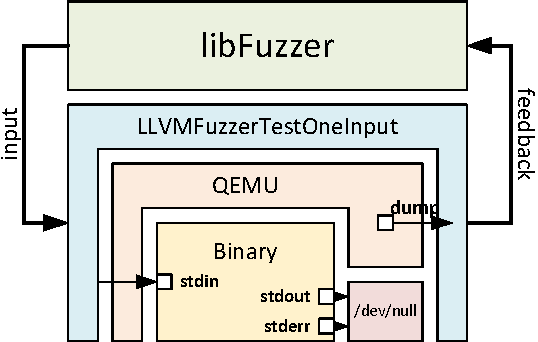
\includegraphics[width=.60\columnwidth]{images/arch.pdf}
\caption{The architecture of our design and implementation.}
\label{fig:arch}
\end{figure}

The architecture of \sys is illustrated in Figure~\ref{fig:arch}.
\sys is implemented as a standalone program and is linked against \libfuzzer.
As a result, \sys contains the ``\libfuzzer" and ``LLVMFuzzerTestOneInput" parts shown in the figure.
To simplify our implementation and maintain program tracing performance, we leverage the QEMU~\cite{qemu} program emulator.
\sys launches a program to be fuzzed (the ``Binary" in the figure) using QEMU user mode.
% command: qemu-x86_64 -D logfile -d in_asm binary
It is worth noting that we disabled the output from the binary launched by QEMU, and patched the QEMU to send required runtime traces to \sys.
%
Once we have done the setup and run the program, test inputs fed by \libfuzzer can be forwarded to the program under test via its standard input.
Program runtime traces reported from QEMU are then used to update internal states required by \libfuzzer.

\subsection{LLVM Hooks}
\label{lbl:hooks}

\libfuzzer leverages LLVM hooks to collect and update program runtime states. To be more specific, the important runtime states collected via hooks includes 1)~coverage, 2)~indirect function calls, 3)~memory search, 4)~comparison, and 5)~address sanitizer~\cite{addresssanitizer}.
%\libfuzzer leverages LLVM hooks to collect and update program runtime states. To be more specific, the important runtime states collected via hooks are listed below.
%\begin{enumerate}
%\item Coverage counter: This is a critical feature used by many grey-box fuzzers. Coverage can be measured in different ways. For example, instruction coverage, block coverage, or edge coverage.
%\item Indirect function calls: Indirect call is a function call to a non-constant address. For example, a function call to a function pointer is an indirection call. The address of a target function can be placed in either a register or a memory address.
%\item Memory search: \libfuzzer also collect the use of memory search relevant functions such as \ttstyle{memmem} and \ttstyle{strstr}.
%\item Comparison: Comparison operations, e.g., \ttstyle{cmp}, may provide hints for the fuzzer to mutate test inputs. Although it may be used to generate interesting test inputs, it could seriously degrade the over testing performance even if it is instrumented at the compiler level.
%\item Address sanitizer: Address sanitizer~\cite{} is an important feature for detecting incorrect or improper memory usage. With address sanitizer, a misbehaved program behavior can be detected without crashing the program.
%\end{enumerate}
For the details about the hooks, readers can refer to LLVM and \libfuzzer documents.
In a fuzzing process, users can choose which states should be collected and used to direct the fuzzing process. However, the coverage counter is the minimum requirement and is used by most grey-box fuzzers.
\sys is a work-in-progress and currently, only the first three items are collected.

%\subsection{Link IO together}
%
%Normally, when using \libfuzzer, we put the source code need to be tested inside \texttt{LLVMFuzzerTestOneInput} as describe in the introduction section.
%But when we want to run a binary, we don't have the source code.
%Hence, what we do is actually putting \texttt{execv("our-binary", ..., ...)} inside the \texttt{LLVMFuzzerTestOneInput} to invoke our binary.
%And before execute \texttt{execv} we need to use dup2 to link
%
%\begin{enumerate}
%  \item [1.] fuzzer test input $\to$ binary stdin.
%  \item [2.] binary stdout $\to$ \texttt{/dev/null}.
%  \item [3.] binary stderr $\to$ \texttt{/dev/null}
%\end{enumerate}
%
%The simplified code is something like below
%
%\begin{lstlisting}[language = c++]
%extern "C" int LLVMFuzzerTestOneInput(const uint8_t *Data, size_t Size) {
%
%    int P_IN[2]; pipe(P_IN);
%    if(Size) write(P_IN[1], Data, Size);
%    ...
%    int pid = fork();
%    if(pid == 0) {
%        dup2(P_IN[0], STDIN_FILENO);
%        dup2(dev_null, STDOUT_FILENO);
%        dup2(dev_null, STDERR_FILENO);
%        ...
%        execv(..., ..., ...);
%    }
%    ...
%}
%\end{lstlisting}

\subsection{Runtime State Collection}
\label{lbl:runtime}

We introduce how runtime state collection and \libfuzzer \libfuzzer-state updating are implemented in \sys.
We receive runtime trace dumps from QEMU user mode, parse the output, and update states required by \libfuzzer.
Currently, we update runtime states in terms of coverage, indirect calls, and memory searches.

\paragraph{Coverage} \libfuzzer uses two arrays to store runtime code coverage, i.e., the \ttstyle{\_\_sancov\_trace\_pc\_pcs} and the \ttstyle{\_\_sancov\_trace\_pc\_guard\_8bit\_counters} arrays.
The former stores the program counter of the beginning of a code block, and the latter stores how many times a code block is visited.
%The pseudocode below demonstrated how the two arrays are updated.
%
%\begin{lstlisting}
%__sancov_trace_pc_pcs[Idx] = PC;
%__sancov_trace_pc_guard_8bit_counters[Idx]++;
%\end{lstlisting}
%
%\noindent
To simplify the identification of basic blocks, we leverage the radare2 api \ttstyle{r2pipe} to perform static analysis and index basic blocks.
With the identified basic blocks within a program under testing, \sys focuses only on fuzzing the program and skip code segments that are irrelevant to the program, e.g., library codes.

%We need to fill those array for LibFuzzer to work.
%First, we use radare2 api \textbf{r2pipe} to do static analysis and index those code block.
%While doing static analysis with r2pipe, we filter out addresses we don't want, like library code.
%Second, we use QEMU to check whether we hit a code block and fill in those value.
%The QEMU command we use is \texttt{qemu-x86\_64 -D logfile -d in\_asm binary}.
%\texttt{in\_asm} provides us the assembly code and its address being executed. ( see example below )
%
%\begin{lstlisting}
%...
%----------------
%IN:
%0x0000004000802c90:  mov    %r11,%rcx
%0x0000004000802c93:  sub    %rax,%rcx
%0x0000004000802c96:  cmp    $0xb,%rcx
%0x0000004000802c9a:  ja     0x4000802dd8
%...
%\end{lstlisting}
%
%After parsing QEMU output and fill in those value, LibFuzzer is now runnable.

\paragraph{Indirect Calls} An indirect call is a function call to a non-constant function address. For example, function call based on a function pointer is an indirection call. The address of a target function can be placed in either a register or a memory address. \libfuzzer collect indirect calls by using the \ttstyle{\_\_sanitizer\_cov\_trace\_pc\_indir} hook function. This function requires the address before a call and the address after the call. To collect the states, we patched QEMU to determine if the end of a basic block is a \ttstyle{call} instruction and the address of the called target. If the target is a register or a memory address, we pass the end address of the current block and the beginning address of the next block to the hook function.

%\subsubsection{trace pc indir}
%
%Indirect call is a call instruction with a nonconstant address.
%For example, \texttt{call rax}.
%Libfuzzer will gather states for indirect call using \texttt{\_\_sanitizer\_cov\_trace\_pc\_indir} hook function.
%It needs the address before a call, and the address after a call.
%We implement this hook function in the following steps.
%
%\begin{enumerate}
%    \item [1.] Modify QEMU source code to output a text message when there is an indirect call.
%    \item [2.] When current translation block has an indirect call, we look at the ending address of the current block and the beginning address of the next block, then pass those values to \texttt{fuzzer::TPC.HandleCallerCallee}
%\end{enumerate}

\paragraph{Memory search}
\libfuzzer also collect the use of memory search relevant functions such as \ttstyle{memmem} and \ttstyle{strstr}. Identifying function calls to interesting functions are similar to identifying indirection calls. The only difference is that \sys has to determine if a target function address is an interested function. This is simple for dynamically linked objects because we would be able to determine the functions from the \ttstyle{plt} table. However, it could be difficult if the program is statically linked against the C library.

